\section{Entwicklung zur DevOps-Kultur} \label{entwicklung}

\subsection{Umsetzung von Continuous Delivery}
Continuous Delivery ist vor allem eine technische Praktik. Trotzdem hat diese Disziplin verschiedene Auswirkungen auf die Organisation. Continuous Delivery steht und fällt mit der Pipeline. Das Umsetzen einer einfachen Delivery-Pipeline kann bereits mit simplen mitteln erfolgen. Vor allem zu Beginn eines Projekts kann der Aufbau einer solchen Pipeline verfolgt werden. Beispielsweise kann ein Unternehmen hier vorab mit den Phasen Commit und Deploy beginnen, da diese schließlich existieren müssen. Es ist dann möglich, die Pipeline im weiteren Verlauf schrittweise weiterzuentwickeln, indem entsprechende Phasen (z. B. automatisierte Tests) hinzugefügt werden. Wird Continuous Delivery zum Start eines Projekts eingeführt, kann dies auch bei der Auswahl der Technologien und Architekturen berücksichtigt werden \cite{Wolff.2016} 
Oft setzt Continuous Delivery allerdings an eine bestehende Codebasis an, die nicht dafür konzipiert wurde. In gewisser Weise besteht immer eine Delivery-Pipeline, da es stets einen Prozess zur Auslieferung der Software gibt. Nur kann dieser Prozess sehr komplex sein. Das Ziel von Continuous Delivery ist allerdings einen konstanten Fluss von Features und Codeänderungen durch die Pipeline zu erreichen. Um die bestehende Pipeline entsprechend anzupassen können verschiedene Ansätze wie beispielsweise Value Stream Mapping angewandt werden. Aus dieser Analysetechnik lassen sich dann Optimierungen ableiten. Zu weiteren Optimierungsmaßnahmen gehört auch DevOps. Value Stream Mapping hingegen wird in dieser Arbeit nicht weiter beleuchtet. 
Beim Übernehmen von Continupus Delivery reicht es allerdings oft nicht, schlicht entsprechende Werkzeuge zu verwenden. Solange die Prozesse innerhalb der Organisation nicht ablaufen, wie bei einer gut geölten Maschine, kann hier keine signifikante Steigerung der Effizienz erreicht werden \cite{Virmani.2015}. Der Schlüssel, um entsprechende Prozesse gut zum Laufen zu bringen ist dabei DevOps. Mit dieser Organisationsform funktioniert Continuous Delivery besonders gut, da hierfür das Wissen aus beiden Abteilungen benötigt wird. Während die Entwicklung die Anwendung, deren Konfiguration und Aufbau kennt, weiß der Betrieb über die Rahmenbedingungen bescheid \cite{Wolff.2016}.

\subsection{Umsetzung von DevOps}
Continuous Delivery ist hauptsächlich mit der DevOps-Bewegung verbunden, da DevOps eine wirkungsvolle Optimierungsmaßnahme darstellt \cite{continuousdelivery.2017}. Dabei fokussiert sich dieser Ansatz auf die Liefergeschwindigkeit, das kontinuierliche Testen in Produktionsähnlichen Umgebungen, kontinuierliche Rückmeldung und schnelle Reaktionsfähigkeit sowie, wie der Name bereits andeutet, das Auflösen der Teamgrenzen \cite{Virmani.2015}. Immerhin sollen die Entwicklung und der Betrieb als eine Einheit agieren und Teams anhand von Komponente oder fachlichen Zuständigkeiten aufgeteilt werden, wodurch auch die vollständige Verantwortung für ein Modul bei dem entsprechenden Team liegt. Damit geht eine Änderung der Organisationsform einher, um eine Kultur und ein Umfeld zu schaffen, indem das Erstellen, Testen und Freigeben von Software schnell, häufig und zuverlässig erfolgen kann. Ein Großteil von DevOps befasst sich demnach mit der Prozessverbesserung durch eine radikale Automatisierung manueller Prozesse \cite{DevOps.2016}.\\ Viele Unternehmen sind bereits dabei, DevOps erfolgreich umzusetzen. Allerdings bleiben nach wie vor kritische Barrieren bei der Entwicklung, wie sie im folgenden Kapitel näher beschrieben werden. Um diese Philosophie anzuwenden gibt es verschiedene Möglichkeiten. Dabei ist vermutlich die größte Hürde die Angst vor Veränderungen (siehe vorherige Abneigung gegenüber Clouds), da etwas Neues auszuprobieren entmutigend sein kann \cite{continuousdelivery.2017}. 
Es muss einem klar sein, was DevOps für das Unternehmen bedeutet. Beim Umsetzen braucht man klar definierte Ziele und einen vereinbarten Zeitrahmen, in welchen diese erreicht werden sollen. Zwei der größten Hindernisse, diese Disziplin erfolgreich umzusetzen, sind die Unternehmensarchitektur sowie Unternehmenskultur, die davon beeinflusst werden.

\subsection{Architektur}
Es werden nun zwei Merkmalen der Unternehmensarchitektur eine hohe Priorisierung zuteil: Testbarkeit und Einsatzfähigkeit. Die Software wird bei Continuous Delivery in einer testbaren Umgebung entwickelt, sodass die meisten Fehler theoretisch direkt vom Entwickler erkannt werden können, indem automatisierte Tests ausgeführt werden. Es sollen keine komplexen Umgebungen mehr aufgesetzt werden, um den Großteil der Akzeptanz- und Regressionstests durchzuführen. Das Design für die Implementierung und die entsprechenden Tests beginnt zudem mit der Sicherstellung, dass die Services aus lose gekoppelten, gut gekapselten Komponenten oder Modulen bestehen (im Rahmen der objektorientierten Programmierung folgen solche Systeme den Prinzipien des SOLID-Designs). Jede Komponente oder jeder Dienst sollte auf Entwicklerarbeitsstationen, Testumgebungen oder in der Produktion vollständig automatisiert bereitgestellt werden können. In einer gut entworfenen Architektur ist es möglich, ein hohes Maß an Vertrauen zu erhalten, dass die Komponente richtig funktioniert, wenn sie auf diese Weise eingesetzt wird. Jede echte serviceorientierte Architektur sollte diese Eigenschaften haben. Die Microservices-Bewegung hat diese architektonischen Eigenschaften sogar explizit priorisiert. Müssen beispielsweise viele Microservices gleichzeitig freigegeben werden („Big Bang-Event“), ist es erforderlich, dass viele Teams in einer sorgfältigen Art und Weise zusammenarbeiten. Solche Bereitstellungen können dabei typischerweise viele Stunden oder sogar Tage in Anspruch nehmen und erfordern eine erhebliche Planung. Auch hier ist die Verbindung zu DevOps wieder erkennbar. Ein Unternehmen muss kontinuierlich und vor allem agil planen. Das setzt voraus, dass es in der Lage ist, sich schnell an die sich ändernden Marktbedingungen anzupassen \cite{continuousdelivery.2017}.
Auch die Unternehmenskultur ist von der Transformation betroffen. Obwohl diese nicht greifbar und nur schwer zu ändern ist, ist es wichtig, eine Kultur zu schaffen, in welcher alle Menschen einer Organisation bei der Verfolgung gemeinsamer Ziele zusammenarbeiten. Dies ging bereits durch den Soziologen Ron Westrum hervor (…), der die Wichtigkeit einer solchen Kultur betonte.
Bei DevOps wird immer die primäre Bedeutung der Kultur hervorgehoben, mit besonderem Fokus auf einer effektiven Zusammenarbeit zwischen Entwicklungsteams und IT-Betriebsteams. Die Forschung zeigt, dass eine Win-Win-Beziehung zwischen Entwicklung und Operation ein signifikanter Prädiktor für die IT-Leistung ist. 
Tatsächlich warten die leistungsstärksten Unternehmen nicht darauf, dass schlimme Dinge passieren, um zu lernen, wie sie sich verbessern können. Sie schaffen regelmäßig (kontrollierte) Unfälle, um schneller zu lernen als die Konkurrenz. Netflix hat dies auf ein neues Level mit ihrer Simian Army gebracht, die ständig ihre Infrastruktur sprengt, um die Ausfallsicherheit ihrer Systeme kontinuierlich zu testen.
Das gemeinsame Thema, das in leistungsstarken Organisationen beobachtet werden kann, ist, dass sie immer versuchen, besser zu werden. 

%\begin{figure}[h!]
%	\centering
%	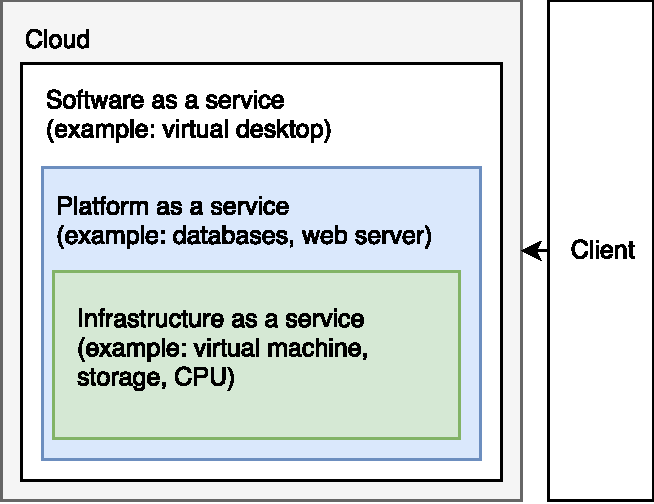
\includegraphics[width=0.8\linewidth]{images/servicemodules.pdf}
%	\caption{Cloud-Servicemodelle} %Generelle
%	\label{fig:cnn_structure}
%\end{figure}